\documentclass{article}

\usepackage{amsmath}
\usepackage{graphicx}

%----------------------------------------------------------------------------------------

\usepackage{listings} % Required for inserting code snippets
\usepackage[usenames,dvipsnames]{color} % Required for specifying custom colors and referring to colors by name

\definecolor{DarkGreen}{rgb}{0.0,0.4,0.0} % Comment color
\definecolor{highlight}{RGB}{255,251,204} % Code highlight color

\lstdefinestyle{Style1}{ % Define a style for your code snippet, multiple definitions can be made if, for example, you wish to insert multiple code snippets using different programming languages into one document
language=c, % Detects keywords, comments, strings, functions, etc for the language specified
backgroundcolor=\color{highlight}, % Set the background color for the snippet - useful for highlighting
basicstyle=\footnotesize\ttfamily, % The default font size and style of the code
breakatwhitespace=false, % If true, only allows line breaks at white space
breaklines=true, % Automatic line breaking (prevents code from protruding outside the box)
captionpos=b, % Sets the caption position: b for bottom; t for top
commentstyle=\usefont{T1}{pcr}{m}{sl}\color{DarkGreen}, % Style of comments within the code - dark green courier font
deletekeywords={}, % If you want to delete any keywords from the current language separate them by commas
%escapeinside={\%}, % This allows you to escape to LaTeX using the character in the bracket
firstnumber=1, % Line numbers begin at line 1
frame=single, % Frame around the code box, value can be: none, leftline, topline, bottomline, lines, single, shadowbox
frameround=tttt, % Rounds the corners of the frame for the top left, top right, bottom left and bottom right positions
keywordstyle=\color{Blue}\bf, % Functions are bold and blue
morekeywords={}, % Add any functions no included by default here separated by commas
numbers=left, % Location of line numbers, can take the values of: none, left, right
numbersep=10pt, % Distance of line numbers from the code box
numberstyle=\tiny\color{Gray}, % Style used for line numbers
rulecolor=\color{black}, % Frame border color
showstringspaces=false, % Don't put marks in string spaces
showtabs=false, % Display tabs in the code as lines
stepnumber=5, % The step distance between line numbers, i.e. how often will lines be numbered
stringstyle=\color{Purple}, % Strings are purple
tabsize=2, % Number of spaces per tab in the code
}

% Create a command to cleanly insert a snippet with the style above anywhere in the document
\newcommand{\insertcode}[2]{\begin{itemize}\item[]\lstinputlisting[caption=#2,label=#1,style=Style1]{#1}\end{itemize}} % The first argument is the script location/filename and the second is a caption for the listing

%----------------------------------------------------------------------------------------


\title{Weekly Report}

\author{}
\date{\today}

\begin{document}

\maketitle

\section{Targets}

\subsection{Urgent}
\begin{itemize}
    \item Randomly selecting a node,
        compute its care set,
        change its care set,
        synthesize the local circuit,
        evaluate its area and error rate,
        accept it with a certain probability.
\end{itemize}

\subsection{Important}
\begin{itemize}
    \item Use approximate confidence interval / hypothesis testing of Bernoulli experiments to evaluate the accuracy of error rate.
    \item Trade off the accuracy of batch error estimation for speed
        (even directly use Su's equation to update Boolean difference),
        perhaps use hypothesis testing to evaluate the accuracy.
    \item Combine the simulation of circuits with the simulation of Monte Carlo Tree Search.
        In other words,
        in one loop of Monte Carlo Tree Search,
        merge logic simulation and playout (only simulate circuit once and playout once).
    \item Represent circuit with AIG because of more potential LAC candidates.
        For each round, select one or more input wires and replace them with constant 0 or 1.
        Consider how to combine Wu's method (choose a subset of input wires and substitute).
    \item Accelerate Approximate Logic Synthesis Ordered by Monte Carlo Tree Search:
        reuse the result of batch error estimation in playout.
    \item How DC affects BDD
    \item Induce DC with PLA files
\end{itemize}

\subsection{Worth Trying}
\begin{itemize}
    \item Enhance default policy with greedy approach or field domain knowledge.
    \item In expansion process of MCTS, expand more than one layers.
    \item Tune parameters in MCTS\@.
    \item Perform greedy flow on leaves of the final Monte Carlo Search Tree.
    \item Combine beam search and MCTS\@.
\end{itemize}

\subsection{Potential Topics}
\begin{itemize}
    \item Relationship between power simulation and logic simulation.
    \item Combine Binarized Neural Network with approximate computing.
    \item Relationship between Boolean network and Bayesian Network.
    \item Approximate TMR\@.
\end{itemize}

\section{Progress}
\subsection{Count \#Literals for Su's work}
See ``./single-selection-result-20190319.xls''

\subsection{Attempt on Don't Care Based ALS}
Currently,
I modify the ``mfs'' command.
The framework is listed below:
\begin{enumerate}
    \item Select a node $f$. (Currently in topological order)
    \item Collect the window for $f$,
        whose inputs are primary inputs $\mathtt x$,
        outputs $\mathtt z$ are nodes in $f$'s fanout cone.
    \item Build a miter $O(\mathtt x)$ for $f$.
    \item Set approximate don't care assignments by change the miter. (which will be discussed later)
    \item Build the SAT problem.
    \item Solve SAT, find interpolation and change the circuit.
    \item If exists other unprocessed node, return to 1.
\end{enumerate}

\begin{center}
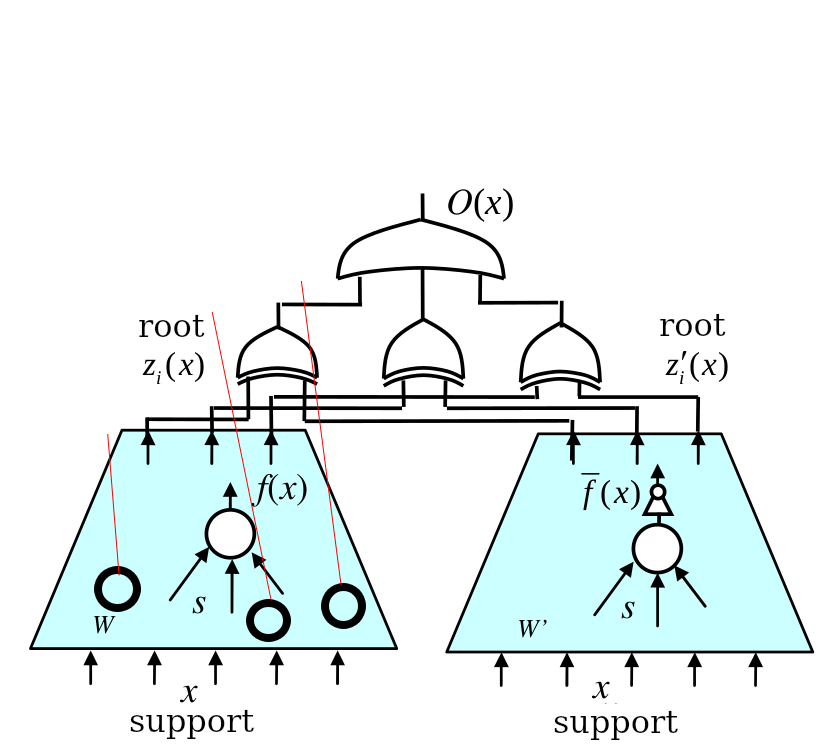
\includegraphics[height=6.5cm]{./miter.png}
\end{center}

\subsection{How to Add Approximate DC assignments}
For a miter,
\[
O(\mathtt x) = 0, \mathtt x \in DC\ set
\]
\[
O(\mathtt x) = 1, \mathtt x \in care\ set
\]

\noindent We want to set an assignment $\hat{\mathtt x} = x_1 x_2 \dots x_n$ as don't care,
where $x_i = 0/1$.

\noindent Then for $\mathtt x = \hat{\mathtt x}$, $\hat{O}(\mathtt x) = 0$,
for $\mathtt x \neq \hat{\mathtt x}$, $\hat{O}(\mathtt x) = O(\mathtt x)$.
So
\[
\hat O(\mathtt x) = \bar{\hat{\mathtt x}} O(\mathtt x)
\]

\subsection{Test on c880}
Since the approximate DCs are directly added on primary inputs,
the number of approximate DCs $m$ decides an upper bound of error rate.
\[
    er \le m / 2^n
\]
where $n$ is the number of primary input.

For c880, $n=26$.

\begin{tabular}{|c|c|c|c|}
    \hline
    m & er & area & time/s\\
    \hline
    0 & 0 &  607 & 0.189\\
    \hline
    1 & 0.000000014 & 589 & 0.207\\
    \hline
    10 & 0.000000149 &594 & 0.241\\
    \hline
    100 & 0.000001490 &553 & 0.595\\
    \hline
    1000 & 0.000014901 &532 & 5.452\\
    \hline
    10000 & 0.000149012 & 408 & 70.104\\
    \hline
\end{tabular}

It seems to be promising,
compared to area of 506 under 5\% error rate in Wu's result.

Time increases as $m$ grows because of the number of clauses in SAT solver increases.
I have two techniques to solve it:
\begin{itemize}
    \item Synthesize the approximate DCs clauses before adding to a solver.
    \item Limit the input of the miter window. (But how to assess the error rate)
\end{itemize}

\end{document}
